\documentclass{article}
\usepackage{amsmath, sfmath, multicol, tkz-euclide, array, enumerate, tcolorbox, tabularray}
\renewcommand{\familydefault}{\sfdefault}
\setlength{\parindent}{0cm}
\pagestyle{empty}
\usepackage[left=1in, top=0.5in, right=1in, bottom=0.5in]{geometry}
\tcbset{colback=white}

\newcounter{example}[section]
\newenvironment{example}[1][]{\refstepcounter{example}\par\medskip
   {\color{red}\textbf{Example~\theexample. #1}}}{\medskip}

\begin{document}

\section*{Measuring Angles}

\begin{tcolorbox}[colframe=orange!70!white, coltitle=black, title=\textbf{Today I Can}]
\begin{enumerate}
    \item Find and compare the measures of angles.
\end{enumerate}
\end{tcolorbox}

\begin{tcolorbox}[
colframe=black!20!white, 
opacitybacktitle=0.1,
coltitle=black, title=\textbf{Angles}]
\textbf{Angles} are formed by 2 rays with the same endpoint. The rays are the \textbf{sides} and the endpoint is the \textbf{vertex}.
\end{tcolorbox}


\vspace{0.25in}

\begin{minipage}{0.55\textwidth}
You can name an angle by
\begin{itemize}
    \item its vertex, $\angle A$
    \item a point on each ray and the vertex, $\angle BAC$ or $\angle CAB$
    \item a number, $\angle 1$
\end{itemize}
\end{minipage}
\hspace{0.25in}
\begin{minipage}{0.4\textwidth}
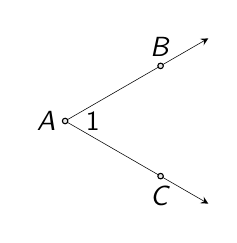
\begin{tikzpicture}[scale=0.7]
    \tkzDefPoints{0/0/A}
    \tkzDefShiftPoint[A](30:2){B}
    \tkzDefShiftPoint[A](-30:2){C}
    \tkzDrawSegment[add = 0 and 0.5, ->, >=stealth](A,B)
    \tkzDrawSegment[add = 0 and 0.5, ->, >=stealth](A,C)
    \tkzDrawPoints(A,B,C)
    \tkzLabelPoints[left](A)
    \tkzLabelPoints[above](B)
    \tkzLabelPoints[below](C)
    \tkzLabelAngle[pos = 0.5](C,A,B){$1$}
\end{tikzpicture}
\end{minipage}
\vspace{0.25in}

The \textbf{sides} of the angle are $\overrightarrow{AB}$ and $\overrightarrow{AC}$. The \textbf{vertex} is $A$.
\newline\\

The \textbf{interior} of an angle is the region containing all of the points between the rays.
\newline\\

The \textbf{exterior} of an angle is all of the points outside the interior.
\newline\\

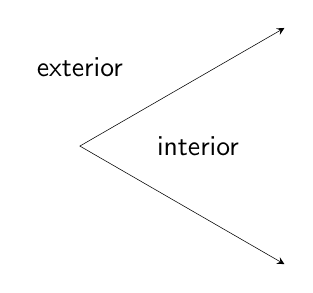
\begin{tikzpicture}
    \tkzDefPoints{0/0/A}
    \tkzDefShiftPoint[A](30:2){B}
    \tkzDefShiftPoint[A](-30:2){C}
    \tkzDrawSegment[add = 0 and 0.5, ->, >=stealth](A,B)
    \tkzDrawSegment[add = 0 and 0.5, ->, >=stealth](A,C)
    \tkzLabelAngle[pos=1.5](C,A,B){interior}
    \node at (0,1) {exterior};
\end{tikzpicture}
\vspace{0.25in}

\begin{example}
Use the diagram below to answer each.
\bigskip 

\begin{minipage}{0.3\textwidth}
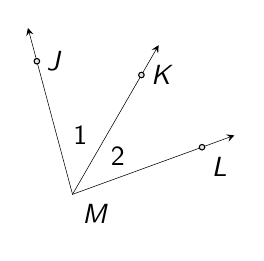
\begin{tikzpicture}
    \tkzDefPoints{0/0/M}
    \tkzDefShiftPoint[M](105:1.75){J}
    \tkzDefShiftPoint[M](60:1.75){K}
    \tkzDefShiftPoint[M](20:1.75){L}
    \tkzDrawSegments[add = 0 and 0.25, ->, >=stealth](M,J M,K M,L)
    \tkzDrawPoints(J,K,L)
    \tkzLabelPoints[right](J,K)
    \tkzLabelPoints[below right](M,L)
    \tkzLabelAngle[pos=0.75](K,M,J){1}
    \tkzLabelAngle[pos=0.75](L,M,K){2}
\end{tikzpicture}
\end{minipage}
\begin{minipage}{0.5\textwidth}
    \begin{enumerate}[(a)]  \setlength{\itemsep}{1.5cm}
        \item What are two other names for $\angle 1$?
        \item What are two other names for $\angle KML$?
    \end{enumerate}
\end{minipage}
\end{example}

\vspace{1.5cm}

Angles with the same measure are \textbf{congruent}. We denote congruent angles based on the number of marking arcs drawn.

\begin{center}
\begin{tikzpicture}
    \tkzDefPoints{0/0/A, 2/0/B}
    \tkzDefShiftPoint[A](40:2){C}
    \tkzDrawSegments[->, >=stealth](A,B A,C)
    \tkzLabelPoints[left](A)
    \tkzMarkAngle[size=0.5](B,A,C)
\end{tikzpicture}
\hspace{0.5in}
\begin{tikzpicture}
    \tkzDefPoints{0/0/A, 2/0/B}
    \tkzDefShiftPoint[A](40:2){C}
    \tkzDrawSegments[->, >=stealth](A,B A,C)
    %\tkzLabelPoints[left](A){$B$}
    \tkzMarkAngle[size=0.5](B,A,C)
    \tkzLabelAngle[pos=-0.25](B,A,C){$B$}
\end{tikzpicture}  
\end{center}
\begin{align*}
    m\angle A &= m\angle B  \\
    \angle A &\cong \angle B
\end{align*}

\begin{example}
Use the figure to fill in the missing value.
\newline\\

\begin{minipage}{0.4\textwidth}
\begin{enumerate}[(a)]  \setlength{\itemsep}{1.5cm}
    \item $\angle LMK \cong$
    \item $\angle IGN \cong$
    \item $\angle RMP \cong$
\end{enumerate}
\end{minipage}
\begin{minipage}{0.7\textwidth}
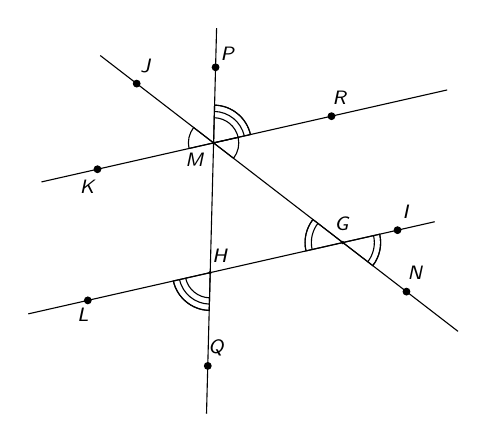
\begin{tikzpicture}[scale=0.8]
\draw [shift={(0.9524041328051618,3.159458079797444)}] (0,0) -- (142.3675785601059:0.4) arc (142.3675785601059:192.77349910381227:0.4) -- cycle;
\draw [shift={(0.9524041328051618,3.159458079797444)}] (0,0) -- (-37.63242143989409:0.4) arc (-37.63242143989409:12.773499103812204:0.4) -- cycle;
\draw [shift={(0.9524041328051618,3.159458079797444)}] (0,0) -- (12.773499103812197:0.6) arc (12.773499103812197:88.50241226098248:0.6) -- cycle;
\draw [shift={(0.8985630736392743,1.100037566702241)}] (0,0) -- (-167.2265008961878:0.6) arc (-167.2265008961878:-91.49758773901755:0.6) -- cycle;
\draw [shift={(3.0043099408008302,1.57742738441278)}] (0,0) -- (-37.63242143989412:0.6) arc (-37.63242143989412:12.773499103812243:0.6) -- cycle;
\draw [shift={(3.0043099408008302,1.57742738441278)}] (0,0) -- (142.36757856010593:0.6) arc (142.36757856010593:192.7734991038122:0.6) -- cycle;
\draw (1.,4.98)-- (0.84,-1.14);
\draw (-1.78,2.54)-- (4.66,4.);
\draw (-1.9902301599211032,0.44512481499445367)-- (4.462707379638399,1.9080578596771978);
\draw (-0.8468806902748067,4.546716602464624)-- (4.832413823626125,0.1679492077285536);
\draw [shift={(0.9524041328051618,3.159458079797444)}] (12.773499103812197:0.6) arc (12.773499103812197:88.50241226098248:0.6);
\draw [shift={(0.9524041328051618,3.159458079797444)}] (12.773499103812197:0.5) arc (12.773499103812197:88.50241226098248:0.5);
\draw [shift={(0.9524041328051618,3.159458079797444)}] (12.773499103812197:0.4) arc (12.773499103812197:88.50241226098248:0.4);
\draw [shift={(0.8985630736392743,1.100037566702241)}] (-167.2265008961878:0.6) arc (-167.2265008961878:-91.49758773901755:0.6);
\draw [shift={(0.8985630736392743,1.100037566702241)}] (-167.2265008961878:0.5) arc (-167.2265008961878:-91.49758773901755:0.5);
\draw [shift={(0.8985630736392743,1.100037566702241)}] (-167.2265008961878:0.4) arc (-167.2265008961878:-91.49758773901755:0.4);
\draw [shift={(3.0043099408008302,1.57742738441278)}] (-37.63242143989412:0.6) arc (-37.63242143989412:12.773499103812243:0.6);
\draw [shift={(3.0043099408008302,1.57742738441278)}] (-37.63242143989412:0.5) arc (-37.63242143989412:12.773499103812243:0.5);
\draw [shift={(3.0043099408008302,1.57742738441278)}] (142.36757856010593:0.6) arc (142.36757856010593:192.7734991038122:0.6);
\draw [shift={(3.0043099408008302,1.57742738441278)}] (142.36757856010593:0.5) arc (142.36757856010593:192.7734991038122:0.5);
\begin{scriptsize}
\draw [fill=black] (0.9837882604055497,4.359900960512274) circle (1.5pt);
\draw[color=black] (1.18,4.57) node {$P$};
\draw [fill=black] (2.8236964398741433,3.583695155623641) circle (1.5pt);
\draw[color=black] (2.96,3.87) node {$R$};
\draw [fill=black] (3.8722475262264204,1.7741958432204452) circle (1.5pt);
\draw[color=black] (4.02,2.07) node {$I$};
\draw [fill=black] (4.014383302021494,0.7986552517862973) circle (1.5pt);
\draw[color=black] (4.16,1.09) node {$N$};
\draw [fill=black] (0.8598557097118462,-0.3805191035218787) circle (1.5pt);
\draw[color=black] (1.,-0.09) node {$Q$};
\draw [fill=black] (-1.044431035046088,0.6595451134909633) circle (1.5pt);
\draw[color=black] (-1.12,0.43) node {$L$};
\draw [fill=black] (-0.891267830442241,2.7414827589370074) circle (1.5pt);
\draw[color=black] (-1.04,2.47) node {$K$};
\draw [fill=black] (-0.26853570513602965,4.1008094290232275) circle (1.5pt);
\draw[color=black] (-0.12,4.39) node {$J$};
\draw [fill=black] (0.9524041328051618,3.159458079797444) circle (0.5pt);
\draw[color=black] (0.66,2.89) node {$M$};
\draw [fill=black] (0.8985630736392743,1.100037566702241) circle (0.5pt);
\draw[color=black] (1.06,1.37) node {$H$};
\draw [fill=black] (3.0043099408008302,1.57742738441278) circle (0.5pt);
\draw[color=black] (3.,1.87) node {$G$};
\end{scriptsize}
\end{tikzpicture}
\end{minipage}
\end{example}
\vspace{0.5in}

\begin{tcolorbox}[
colframe=black!20!white, 
opacitybacktitle=0.1,
coltitle=black, title=\textbf{Angle Addition Postulate}]
If $B$ is in the interior of $\angle AOC$ then $m\angle AOB + m\angle BOC = m\angle AOC$.

\begin{center}
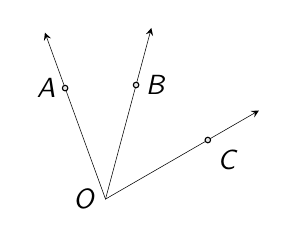
\begin{tikzpicture}
    \tkzDefPoints{0/0/O}
    \tkzDefShiftPoint[O](110:1.5){A}
    \tkzDefShiftPoint[O](75:1.5){B}
    \tkzDefShiftPoint[O](30:1.5){C}
    \tkzDrawSegments[add = 0 and 0.5, ->, >=stealth](O,A O,B O,C)
    \tkzDrawPoints(A,B,C)
    \tkzLabelPoints[left](A,O)
    \tkzLabelPoints[right](B)
    \tkzLabelPoints[below right](C)
\end{tikzpicture}
\end{center}
\end{tcolorbox}



\vspace{0.25in}

\begin{example}
Find the measure of each angle. \bigskip 

\begin{tabular}{p{0.33\textwidth}p{0.33\textwidth}p{0.33\textwidth}}
(a)  $m\angle LKN = 145^\circ$  &
(b)  $\overleftrightarrow{KM}$    &
(c)     \\[0.2in]
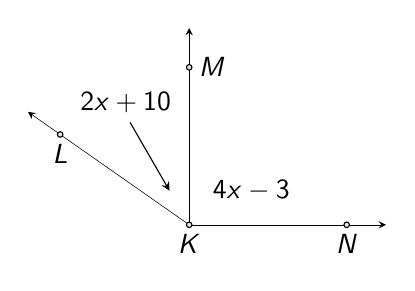
\begin{tikzpicture}
    \tkzDefPoints{0/0/K, 2/0/N}
    \tkzDefShiftPoint[K](90:2){M}
    \tkzDefShiftPoint[K](145:2){L}
    \tkzDrawSegments[add = 0 and 0.25, ->, >=stealth](K,N K,M K,L)
    \tkzDrawPoints(K,L,M,N)
    \tkzLabelPoints[below](L,K,N)
    \tkzLabelPoints[right](M)
    \tkzLabelAngle[pos=0.25, above right](N,K,M){$4x-3$}
    \tkzLabelAngle[pos=1.75](M,K,L){$2x+10$}
    \draw [->, >=stealth](120:1.5) -- (120:0.5);
\end{tikzpicture}
&
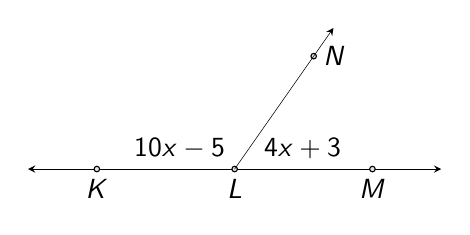
\begin{tikzpicture}
    \tkzDefPoints{0/0/L, 1.75/0/M, -1.75/0/K}
    \tkzDefShiftPoint[L](55:1.75){N}
    \tkzDrawSegment[add = 0.25 and 0.25, <->, >=stealth](K,M)
    \tkzLabelPoints[below](K,L,M)
    \tkzDrawPoints(K,L,M,N)
    \tkzLabelPoints[right](N)
    \tkzDrawSegment[add = 0 and 0.25, ->, >=stealth](L,N)
    \node at (0,0) [anchor = south east] {$10x-5$};
    \node at (0.25,0) [anchor = south west] {$4x+3$};
\end{tikzpicture}
&
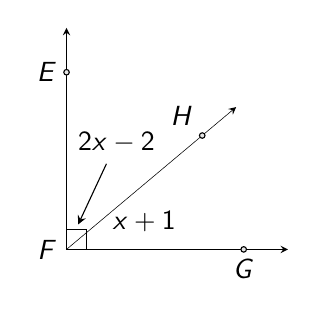
\begin{tikzpicture}
    \tkzDefPoints{0/0/F, 2.25/0/G, 0/2.25/E}
    \tkzDefShiftPoint[F](40:2.25){H}
    \tkzDrawSegments[add = 0 and 0.25, ->, >=stealth](F,G F,H F,E)
    \tkzDrawPoints(E,H,G)
    \tkzLabelPoints[left](E,F)
    \tkzLabelPoints[above left](H)
    \tkzLabelPoints[below](G)
    \tkzMarkRightAngle(G,F,E)
    \tkzLabelAngle[pos=1.05](G,F,H){$x+1$}
    \tkzLabelAngle[pos=1.5](H,F,E){$2x-2$}
    \draw[->, >=stealth] (65:1.2) -- (65:0.35);
\end{tikzpicture}
\end{tabular}
\end{example}

\end{document}
